\documentclass[aspectratio=169,11pt]{beamer}
\usefonttheme{serif}
\mode<presentation>{
    \usetheme{Madrid}
    \useoutertheme{infolines} % Alternatively: miniframes, infolines, split
    % \useinnertheme{circles}
    \definecolor{DarkedRed}{RGB}{167,38,47} % UBC Blue (primary)
    \usecolortheme[named=DarkedRed]{structure}
    \setbeamercolor{palette secondary}{bg=DarkedRed!90!white,fg=white}
    \setbeamercolor{palette tertiary}{bg=black,fg=white}
}
\usepackage{graphicx}
\usepackage{mathtools}
\usepackage{bookmark}
\usepackage{booktabs}
\usepackage{amsthm}
\usepackage{tabulary}
\DeclareMathOperator*{\argmax}{argmax}
\DeclareMathOperator*{\argmin}{argmin}

\title[Quant]{Quantitative Trading Strategies} % The short title appears at the bottom of every slide, the full title is only on the title page

\author[Diego Zhu]{Haixiang Zhu} % Your name
\institute[] % Your institution as it will appear on the bottom of every slide, may be shorthand to save space
{
\textit{Finance Area, Department of Economics, Stony Brook University}  \\ % Your institution for the title page
\medskip\medskip
% \textit{haixiang.zhu@stonybrook.edu} \\% Your email address

\includegraphics[width=0.5\linewidth]{SBU_CoArtsSciences.jpg}
}
\date[DoE Stony Brook]{} % Date, can be changed to a custom date
\setbeamertemplate{navigation symbols}{}
\setbeamercovered{dynamic}
\setbeamertemplate{section in toc}{\inserttocsection}
\setbeamertemplate{section in toc shaded}[default][50]
\AtBeginSection[]
{
  \begin{frame}{Quantitative Trading}
    \tableofcontents[currentsection]
  \end{frame}
}
\begin{document}
    \setbeamertemplate{headline}{}
    \setbeamertemplate{footline}{}
    \begin{frame}
        \titlepage
    \end{frame}
    \setbeamertemplate{footline}[infolines theme]
    
    \begin{frame}
        \frametitle{Outline}
        \tableofcontents
    \end{frame}

    \section{A Brief History}
    \begin{frame}
        \frametitle{Academia}
        \begin{itemize}
            \item Modern Portfolio Theory (MPT), Markowitz (1952, 1959)
            \item M\&M Theorem, Modigliani and Miller (1958)
            \item CAPM, Sharpe (1964)
            \item Efficient Captial Market, Fama (1970)
            \item B-S Option Pricing Model, Black and Scholes (1973)
            \item Arbitrage Pricing Pheory (APT), Ross (1976)
            \item B-L Gobal Portfolio Optimization Model, Black and Litterman (1992)
            \item FF3, Fama \& French (1993)
            \item FF5, Fama \& French (2015)
        \end{itemize}
    \end{frame}
    \begin{frame}
        \frametitle{Industry: \(\mathbb{P}\) vs. \(\mathbb{Q}\)}
        \centering
        \begin{tabular}{ccc}
            \toprule
            \toprule
            &\textbf{Risk/portfolio management}&\textbf{Derivatives pricing}\\
            \midrule
            Goal&model the future&extrapolate the present\\
            Environment&real probability \(\mathbb{P}\)&risk-neutral probability \(\mathbb{Q}\)\\
            Processes&discrete-time series&continuous-time martingales\\
            Dimension&large&low\\
            Tools&multivariate statistics&Ito calculus, PDE’s\\
            Challenges&estimation&calibration\\
            Business&buy-side&sell-side\\
            \bottomrule
            \bottomrule
            \end{tabular}
    \end{frame}

    \section{Learning Tips}
    \begin{frame}
        \frametitle{Learning Tips}
        \begin{itemize}
            % \item \href{https://blog.lofyer.org/wp-content/uploads/python-quant-uqer.pdf}{Quant Tutorial (python version)}
            % \item \href{https://uqer.datayes.com/}{Uqer}
            % \item \href{https://www.windquant.com/}{Windquant}
            % \item \href{https://www.joinquant.com/}{Joinquant}
            \item \href{https://www.quantconnect.com/}{Quantconnect}: Alternative for Quantopian
            \item \href{https://quantiacs.com/}{Quantiacs}
            \item \href{https://blueshift.quantinsti.com/}{Blueshift}
        \end{itemize}
    \end{frame}

    \begin{frame}{Pipeline}
        \centering
        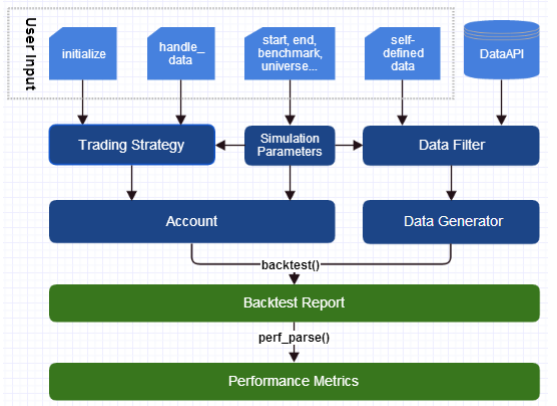
\includegraphics[width=0.6\linewidth]{quant_pipline.png}
    \end{frame}

    \section{Smart Beta Strategy}
    \begin{frame}{Smart Beta}
        Along with the concept of factor/style investing, Smart Beta becomes a hop topic in the last few years.
        \begin{definition}[Smart Beta Strategies]
            Smart beta strategies are designed to add value by systematically selecting, weighting, and rebalancing portfolio holdings on the basis of factors or characteristics other than market capitalization.
        \end{definition}
        Why is it so disruptive to the business of traditional active management?
        \begin{itemize}
            \item simple and rule-based
            \item transparent
            \item lower fees
        \end{itemize}
    \end{frame}

    \begin{frame}{Smart Beta Model}
        \[E(R^e)=\alpha+\beta'\lambda\]
        where
        \begin{align*}
            \lambda&:\text{risk premium}\\
            \beta&:\text{risk exposure}\\
            \alpha&:\text{pricing error}
        \end{align*}
    \end{frame}

    \begin{frame}{Performance of classic factors in China's market (2004/01-2020/10)}
        \centering
        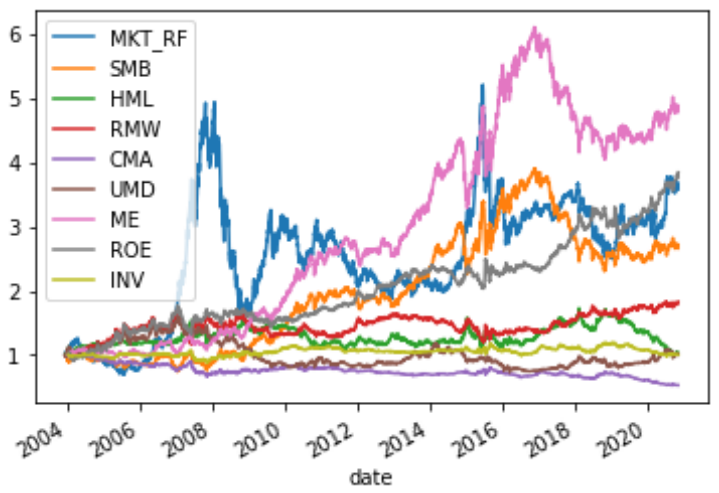
\includegraphics[width=0.6\linewidth]{factors_cn.png}
    \end{frame}

    \begin{frame}
        \frametitle{Descriptive Statistics}
        \centering
        \begin{tabulary}{\linewidth}{cccccccccc}
            \toprule
            \toprule
            &\textbf{MKT\_RF}& \textbf{SMB}& \textbf{HML}& \textbf{RMW}& \textbf{CMA}& \textbf{UMD}& \textbf{ME}& \textbf{ROE}& \textbf{INV}\\
            \midrule
            count& 202& 202& 202& 202& 202& 202 &202& 202& 202\\
            mean& 0.92& 0.64& 0.06& 0.32& -0.28& 0.04& 0.86& 0.73& 0.02\\
            std& 7.98 &4.81 &3.89 &3.46 &2.35& 4 &4.18& 3.47 &2.06\\
            min& -25.14& -20.10& -14.76& -8.72 &-11.69& -13.23 &-19.46 &-9.42& -9.63\\
            25\% &-3.45& -2.30 &-1.94& -1.48 &-1.80 &-2.30 &-1.55 &-1.38 &-1.10\\
            50\%& 1.04& 0.40& 0.05& 0.08& -0.45& 0.03& 0.87 &0.71 &-0.15\\
            75\% &4.87& 3.64& 2.07& 1.95 &1.17 &2.54 &3.51 &2.74 &1.26\\
            max &28.58 &19.36& 19.30 &16.45 &5.69 &13.14& 18.27& 15.24& 6.66\\
            t-stat& 1.65 &1.90& 0.22 &1.32 &-1.70 &0.16 &\alert{2.94} &\alert{2.97}& 0.16\\
            \bottomrule
            \bottomrule
        \end{tabulary}
    \end{frame}
    
    \begin{frame}{How to combine?}
        \begin{itemize}
            \item Reasearch: e.g. Altman's Z-score (1968)
            \begin{align*}
                Z_{score}=&1.2\cdot\frac{\text{Working capital}}{\text{Total assets}}+1.4\cdot\frac{\text{Retained Earnings}}{\text{Total assets}}+3.3\cdot\frac{\text{EBIT}}{\text{Total assets}}\\
                &+0.6\cdot\frac{\text{Market value of equity}}{\text{Book value of total liabilities}}+0.999\cdot\frac{\text{Sales}}{\text{Total assets}}
            \end{align*}
            \item IC: corr(\(\beta_{-1}, R^e\))
            \item IR: \(\dfrac{Mean_{IC}}{Std_{IC}}\)
        \end{itemize}
    \end{frame}

    \section{Asset Allocation Strategy}
    \begin{frame}{Asset Allocation}
        \begin{itemize}
            \item 1952, Markowitz's Mean-Variance optimization (MVO)\\
            Improvement: incoporating macro data to estimate expected return and CVaR as alternative risk measrue
            \item 1990, Fischer Black \& Robert Litterman, Goldman Sachs, B-L Model
            \item 1996, Ray Dalio, Bridgewater, All Weather Strategy\\
            55\% fixed income, 30\% stocks and 15\% real assets
            \item 2005 Edward Qian, PanAgora, Risk Parity Model
        \end{itemize}
    \end{frame}

    \begin{frame}{Risk Parity Model}
        The risk contribution for each asset \(i\) is given by
        \[RC_i=w_i\frac{\partial \sigma_p}{\partial w_i}=w_i\frac{(\sum w)_i}{\sqrt{w'\Sigma w}}\]    
        Solution
        \[\argmin_w\sum_{i=1}^n\left(\frac{\sqrt{w'\Sigma w}}{n}-RC_i\right)^2\]
    \end{frame}

    \begin{frame}{Black-Litterman Model}
        First, consider the implied excess equilibrium return
        \[\Pi=\delta\Sigma\cdot w_{mkt}\]
        where
        \begin{align*}
            \delta&:\text{risk aversion coefficient}\\
            \Sigma&:\text{covariance matrix of excess returns}\\
            w_{mkt}&:\text{market capitalization weight}
        \end{align*}
    \end{frame}

    \begin{frame}{Black-Litterman Model (cont’d)}
        Then compute the posterior expected return
        \[E(R)=[(\tau\Sigma)^{-1}+P'\Omega^{-1}P]^{-1}[(\tau\Sigma)^{-1}\Pi+P'\Omega^{-1}Q]\]
        where
        \begin{align*}
            \tau&:\text{scalar}\\
            P&:\text{view matrix}\\
            Q&:\text{view vector}\\
            \Omega&:\text{diagonal covariance matrix with entries of the uncertainty within each view}
        \end{align*}
    \end{frame}

    \begin{frame}{Black-Litterman Model (cont’d)}
        After that, compute the posterior covariance matrix
        \[\Sigma_p=\Sigma+(\tau\Sigma)^{-1}+P'\Omega^{-1}P]^{-1}\]
        Finally, plugging updated expected return and covariance matrix back in MVO.
    \end{frame}

    \begin{frame}{Market Timing/GTAA}
        Summary of Risky Assets
        \begin{itemize}
            \item U.S. Equity: 10
            \item Global ex U.S. Equity: 19
            \item Fixed Income: 6
            \item Real Assets: 7
        \end{itemize}
        Strategy
        \begin{itemize}
            \item Define signal: \(Signal_t=\dfrac{MAMOM_t(12)}{Vol_t(12)}=\dfrac{\dfrac{P_t}{MA_t(13)}-1}{Std_t(12)}\)
            
            where \(MA_t(13)=Mean(P_t,P_{t-1},\dots,P_{t-12})\)
            \item Portfolio Sort: select top n(15) cross-sectional assets
            \item Risk control (thereshold: 0): remove assets whose signal < 0
        \end{itemize}
    \end{frame}

    \begin{frame}{Market Timing/GTAA (2000/1-2020/9)}
        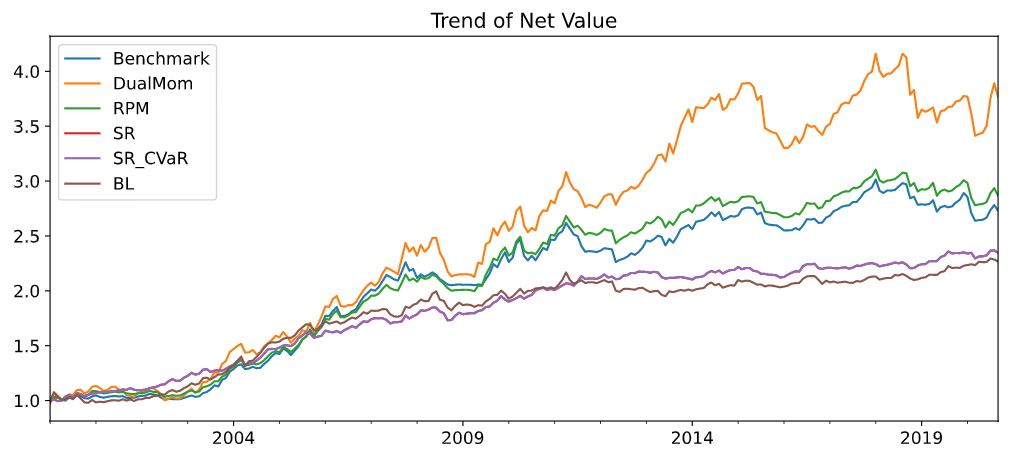
\includegraphics[width=\linewidth]{gtaa_30bps.png}
    \end{frame}

    \section{AI-driven Strategy}
    \begin{frame}{AI-driven}
        \begin{itemize}
            \item Stock Selection
            \item \href{https://github.com/microsoft/qlib}{Qlib}
            \item \href{https://github.com/AI4Finance-LLC/FinRL-Library}{FinRL}
        \end{itemize}
    \end{frame}

    \begin{frame}{Research from HTSC}
        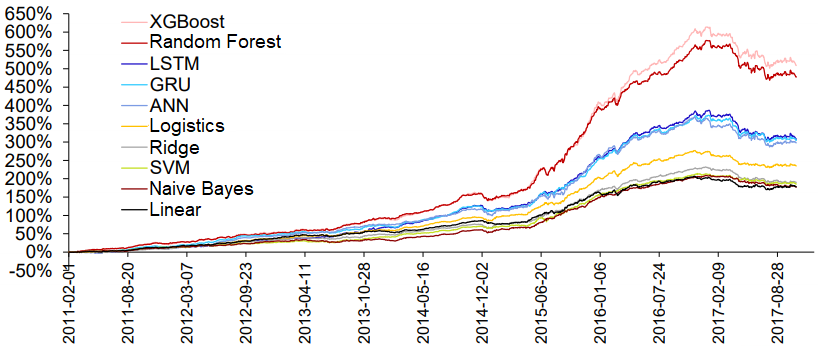
\includegraphics[width=\linewidth]{ml_huatai.png}
    \end{frame}

    \begin{frame}{Feature Selection}
        Total Factors: 72
        \begin{itemize}
            \item Valuation factors: 5
            \item Size factors: 2
            \item Growth factors: 8
            \item Quality factors: 2
            \item Size factors: 8
            \item Leverage factors: 2
            \item Risk factors: 6
            \item Liquidity factors: 6
            \item Technical indicators: 15
            \item Momentum factors: 9
            \item Earnings Expectation: 9
        \end{itemize}
    \end{frame}

    \begin{frame}{Data Cleaning}
        \begin{itemize}
            \item Winsorization: MAD
            \item Normalization: Z-Score
            \item Neutralization: Cap + Style(Industry)
        \end{itemize}
    \end{frame}

    \begin{frame}{2010/1-2020/5}
        \centering
        \begin{tabulary}{\linewidth}{CCCCCC}
            \toprule
            \toprule
            \textbf{Algorithm (lb: Months)}& \textbf{Annualized Return}& \textbf{Benchmark (CSI300)}& \textbf{Excess Return}& \textbf{Sharpe Ratio}& \textbf{Max Drawdown}\\
            \midrule
            LSTM(36)& 27.11\%& 5.51\%& 21.60\%& 0.99& -20.44\%\\
            XGBoost(12)& 18.42\%& 2.25\%& 16.17\%& 0.69& -35.82\%\\
            LR(36)& 19.63\%& 5.51\%& 14.12\%& 0.75& -20.93\%\\
            SVM(12)& 20.89\%& 2.25\%& 18.64\%& 0.77& -37.73\%\\
            GaussianNB(12)& 13.82\%& 2.25\%& 11.57\%& 0.58& -32.57\%\\
            RF(12)& 17.44\%& 2.25\%& 15.19\%& 0.66& -31.57\%\\
            \bottomrule
            \bottomrule
        \end{tabulary}
    \end{frame}

    \begin{frame}{FinRL}
        \centering
        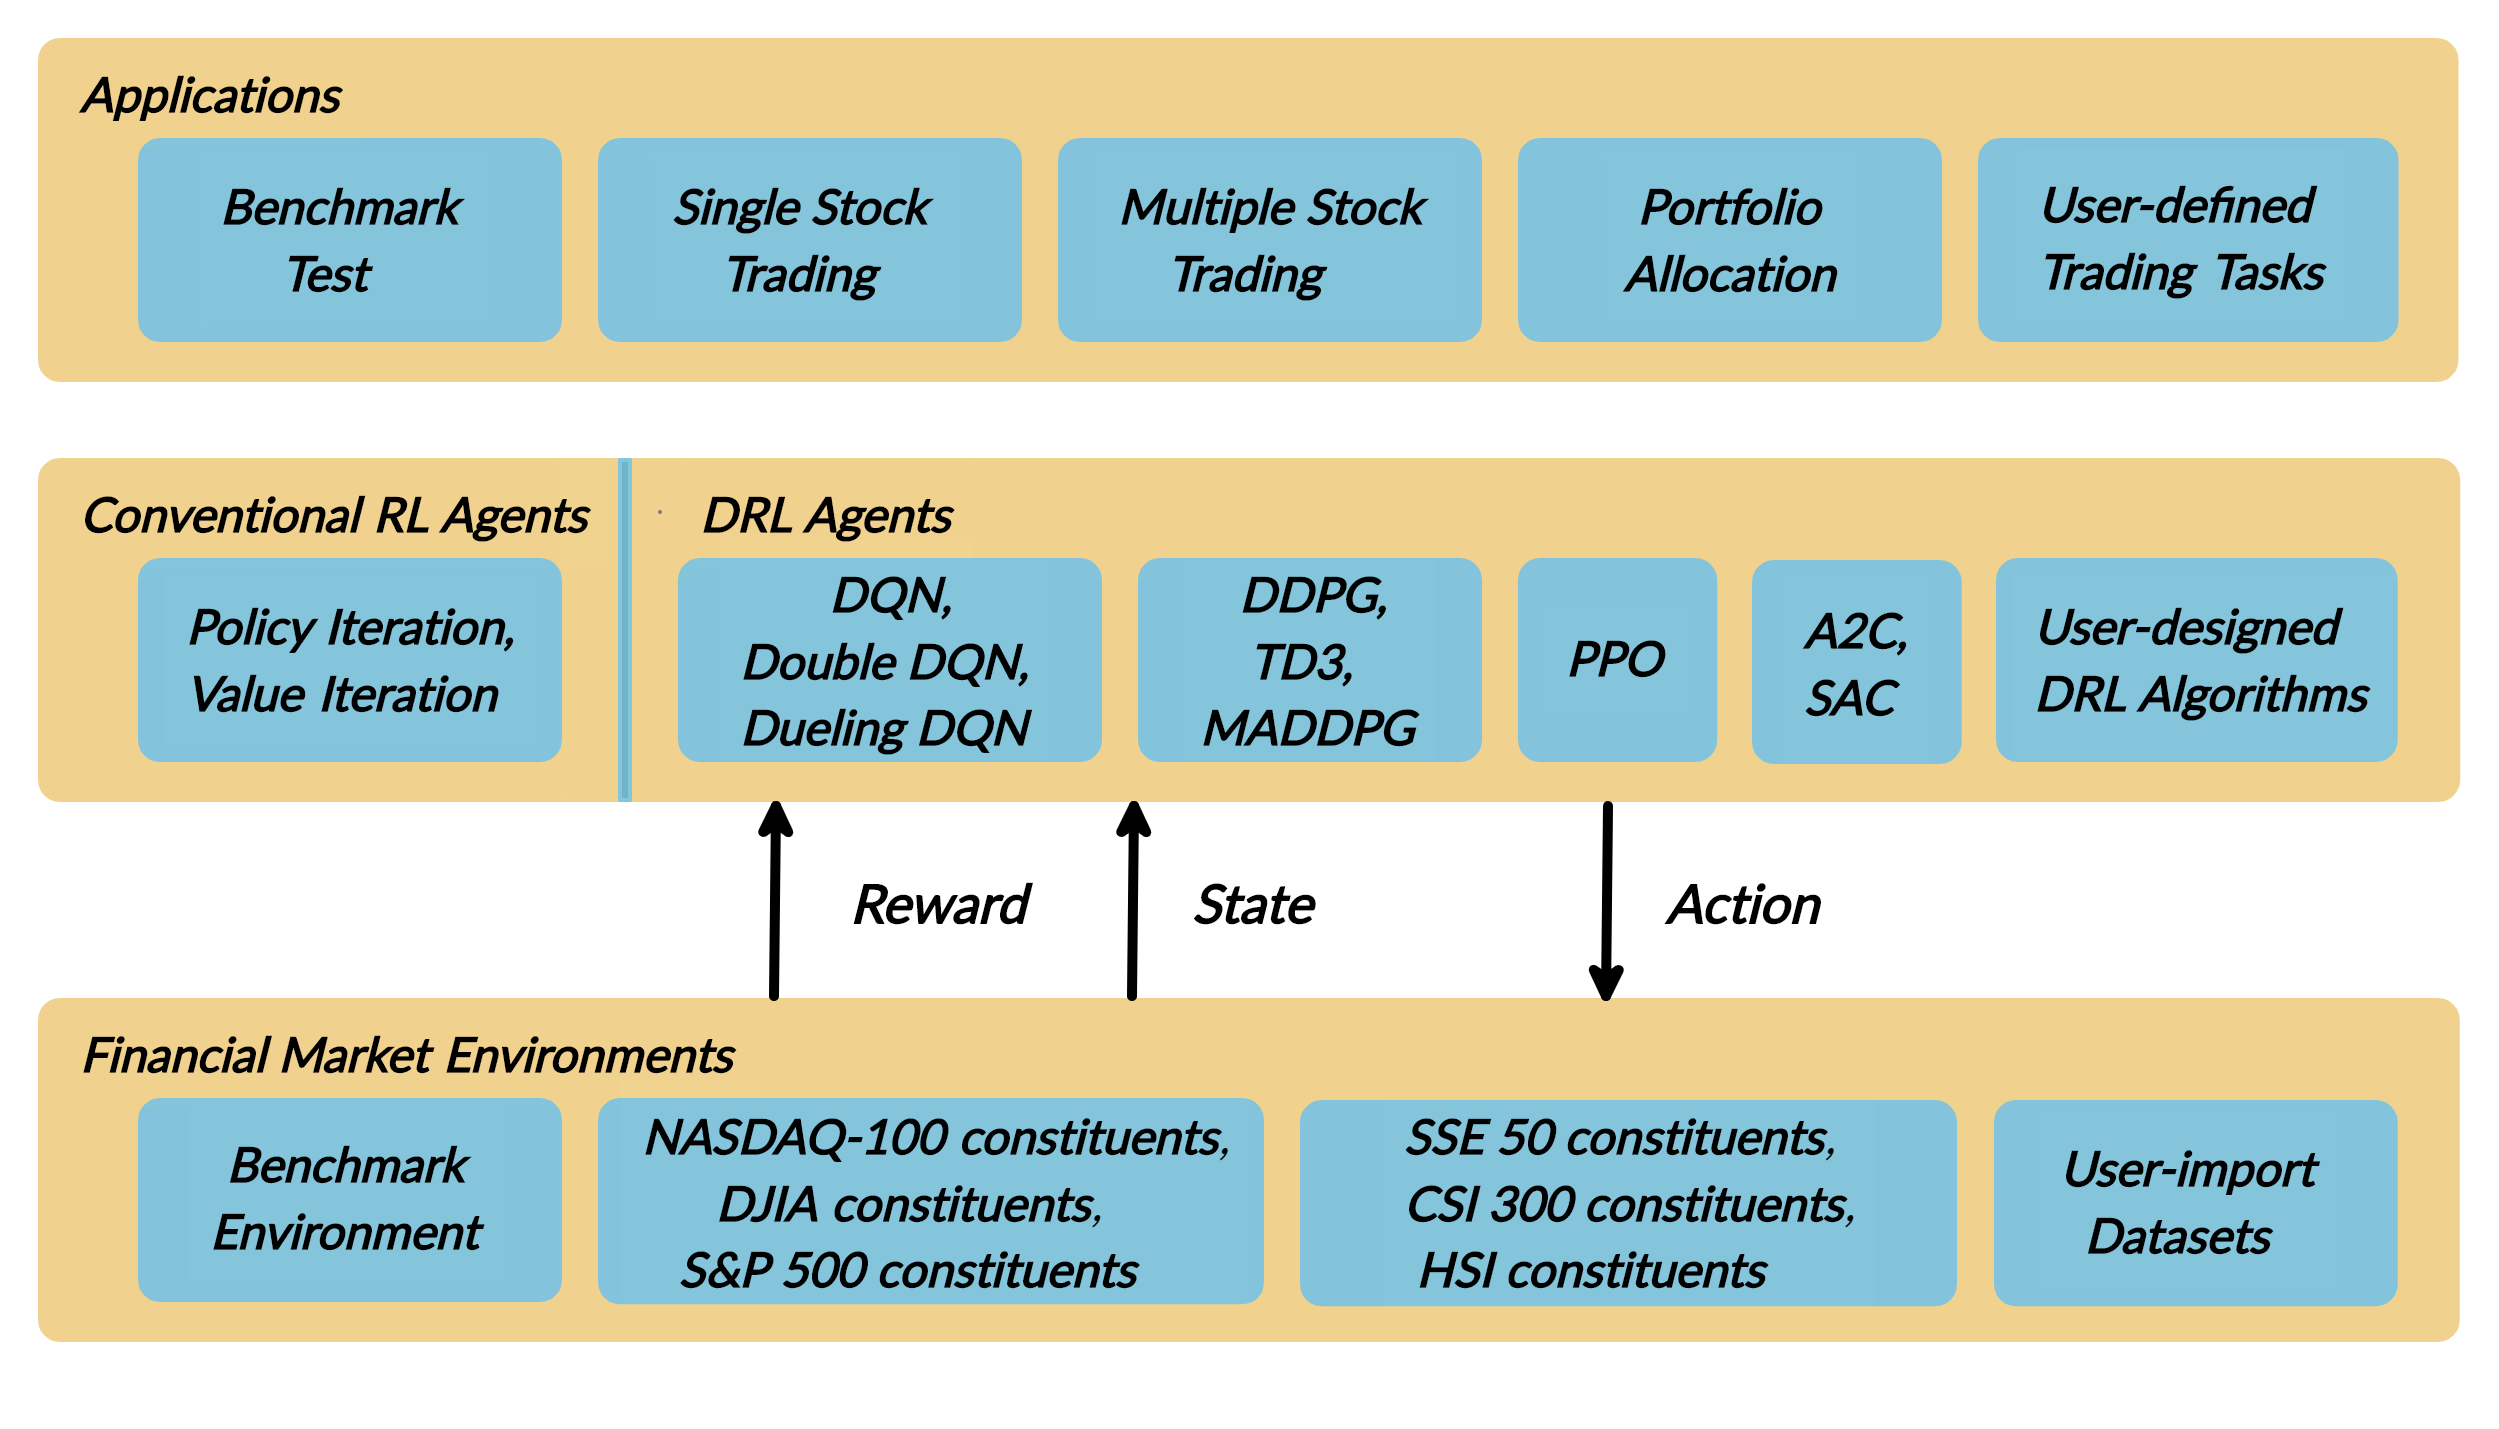
\includegraphics[width=0.8\linewidth]{FinRL-Architecture.png}
    \end{frame}

    \begin{frame}{FinRL}
        \centering
        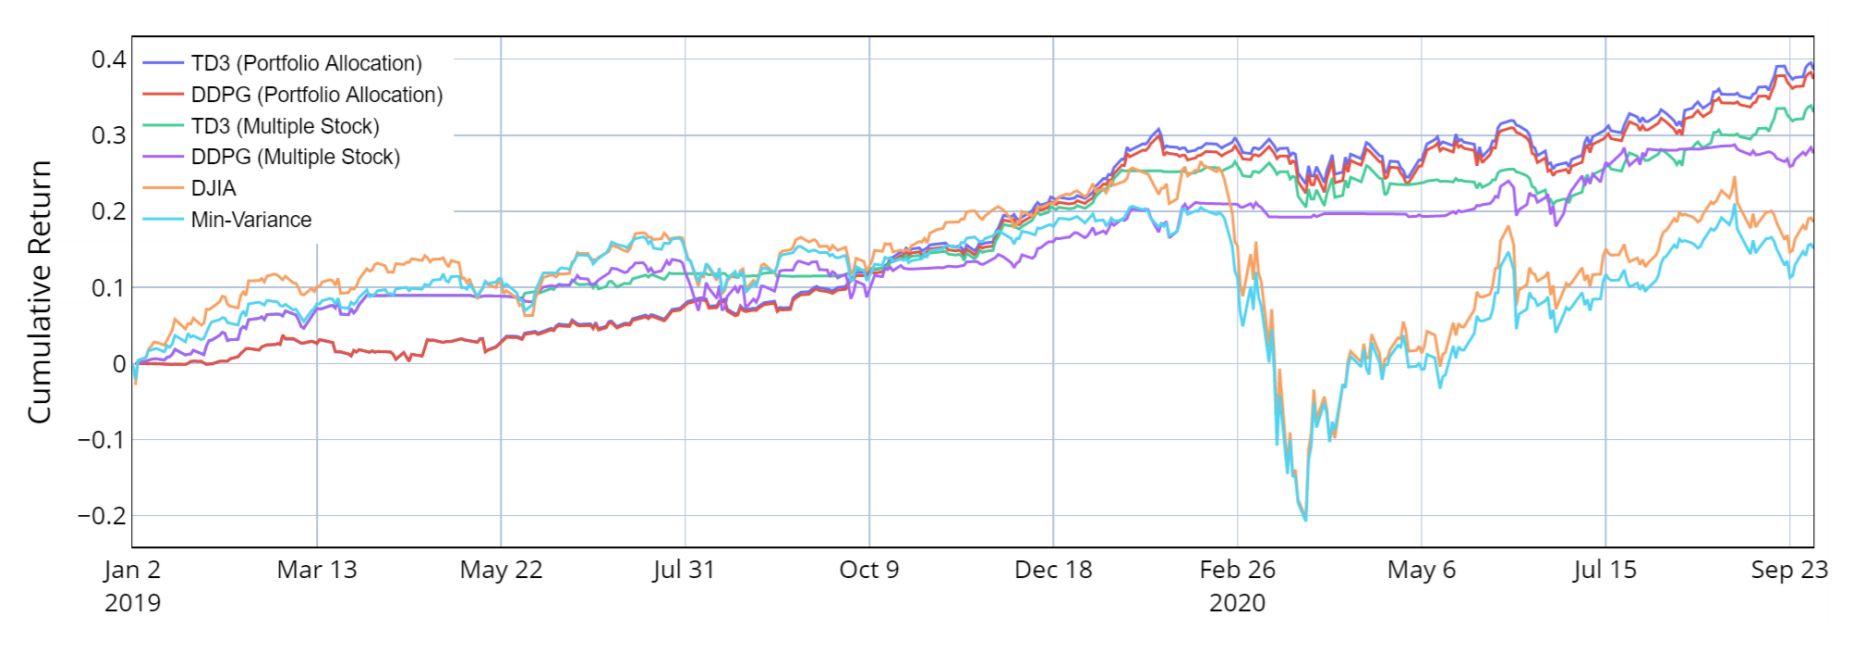
\includegraphics[width=\linewidth]{performance.png}
    \end{frame}
    \begin{frame}{Qlib}
        \centering
        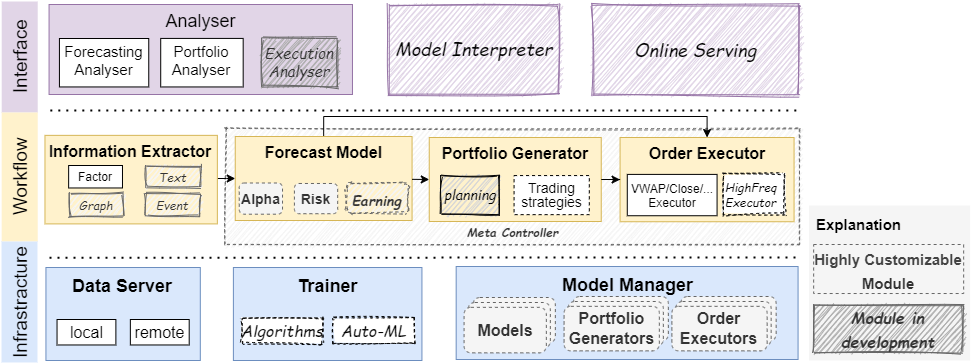
\includegraphics[width=\linewidth]{qlib_framework.png}
    \end{frame}
    \begin{frame}{Qlib}
        \centering
        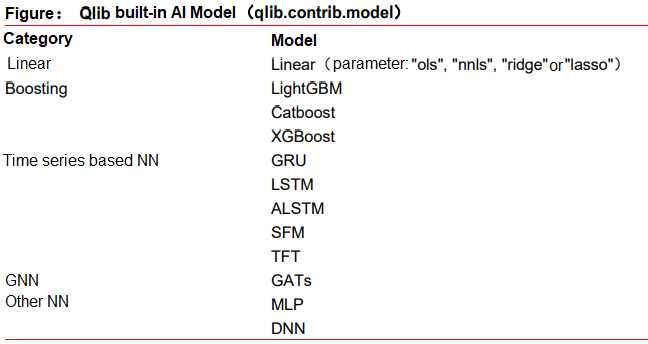
\includegraphics[width=0.8\linewidth]{qlib_model.png}
    \end{frame}
\end{document}